  
  This chapter presents the results for the \acs{us} airline passenger dataset. 
  First, the model specifications and the results using \acs{grl} and \acsp{gnn} 
  are presented. Afterwards, the \acs{gml} results are compared to the results 
  using standard \acs{ml} models. For the comparison, the standard models 
  logistic regression \citep{cramer2002origins}, naive bayes 
  \citep{zhang2004bayes}, \acsp{svm} \citep{platt1999probabilistic,chang2011libsvm}, 
  random forest classifiers \citep{breiman2001random}, AdaBoost classifiers 
  \citep{freund1997decision,hastie2009multi}, \acs{qda}
  \citep{tharwat2016linear}, and \acsp{ann}
  \citep{mcculloch1943logical,werbos1974beyond} are considered.

  \section{Graph Representation Learning}
  \label{section:result_n2v}

  The graph generated in section \ref{section:graph_gen} using the \acs{mag}
  model was used for \acs{grl}. The Node2Vec algorithm using an unbiased walk 
  was employed for learning the 2-dimensional node representations 
  of the graph. The Node2Vec model specifications were set as follows:

  \begin{itemize}
    \setlength\itemsep{0.1em}
    \item Embedding size $d$: 2
    \item Random walk length $t$: 8
    \item Number of random walks $\gamma$: 100
    \item Window size $w$: 10
    \item Node batch size: 2
    \item Return parameter $p=1$
    \item In-out parameter $q=1$
  \end{itemize}

  \noindent With the specified return- and in-out parameters, the Node2Vec
  output corresponds to the DeepWalk output. The resulting node embeddings are
  then used as inputs for standard \acs{ml} models. The node embeddings are 
  shown in figure \ref{fig:node2vec}. 

  \begin{figure}[h]
		\centering
		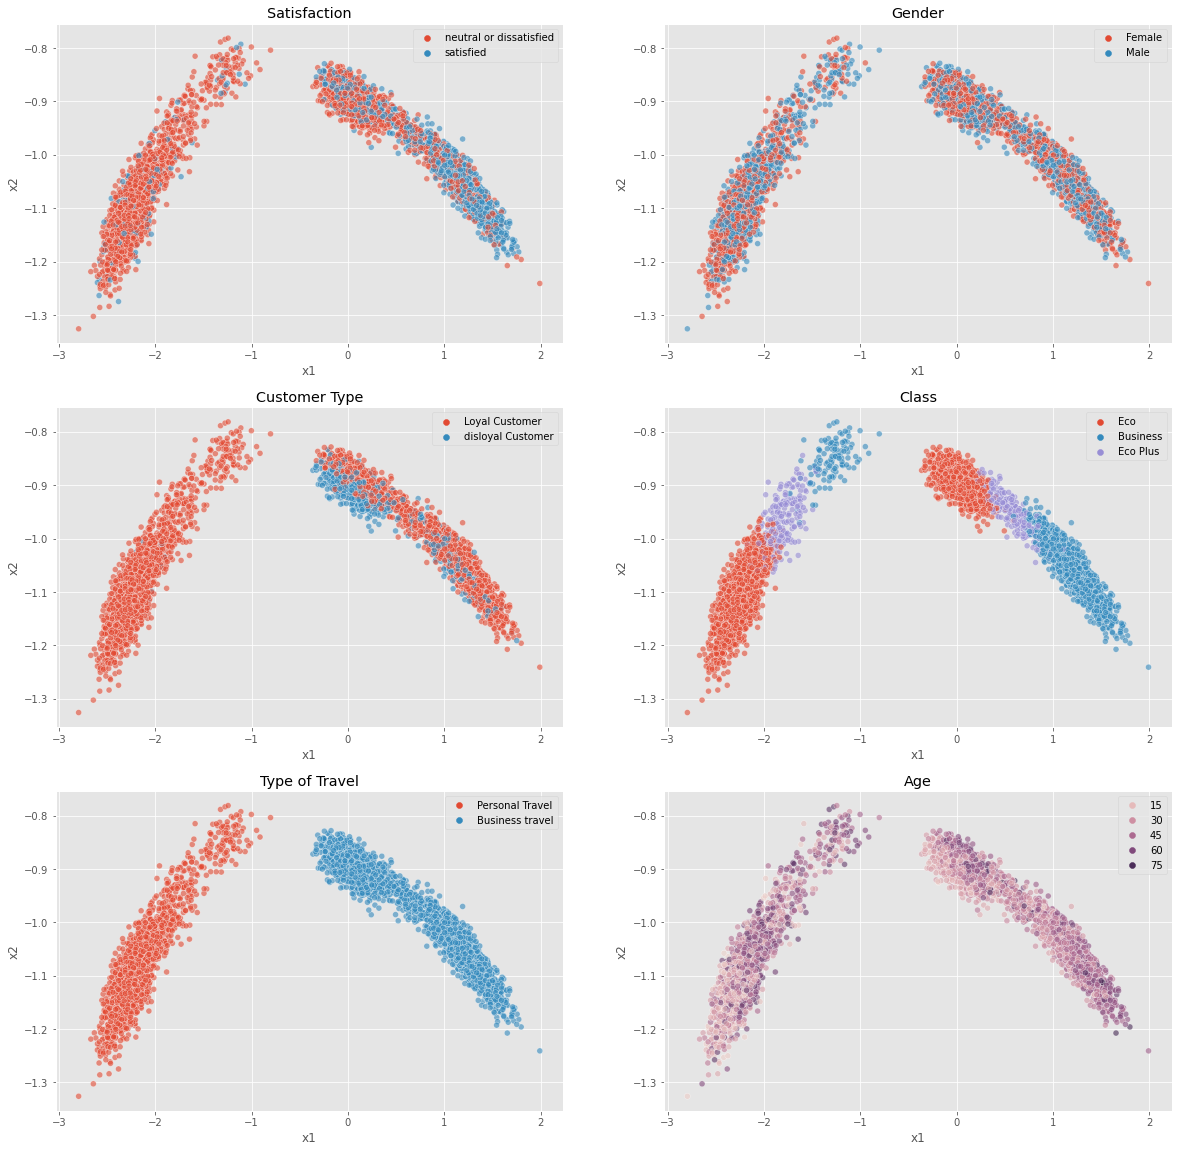
\includegraphics[width=0.9\textwidth]{node2vec_emb.png}
		\caption{Node2Vec Embeddings}
        \label{fig:node2vec}
  \end{figure}

  \noindent The plotted node embeddings in figure \ref{fig:node2vec} reveal 
  interesting neighborhood structures. First, the nodes are split according to
  their type of travel. This corresponds to the two main clusters shown in
  figure \ref{fig:us_airline_graph}. Secondly, the node embeddings are grouped 
  in a nice and orderly fashion. The node embeddings are part of Euclidean
  space, which is why the plots shown in figure \ref{fig:node2vec} are proper
  scatter plots. This allows for a direct comparison of nodes and the groups to
  which they belong to. The 2-dimensional node embeddings are thus useful for
  gaining insights via data visualization.\\

  \noindent The node embeddings are used as input data for the standard \acs{ml} 
  models and are shown in table \ref{table:node2vec_results}.

  \begin{table}[h]
    \centering
    \scalebox{0.85}{
    \begin{tabular}{|l||l|l|l|}
      \hline
      \textbf{ML Method} & \textbf{Training Accuracy} & \textbf{Validation
      Accuracy} & \textbf{Test Accuracy}\\
      \hline\hline
      Logistic Regression & 77.04\% & 76.16\% & 57.05\%  \\\hline 
      Support Vector Machine & 76.71\% & 77.00\% & 39.08\% \\\hline
      ANN & 76.78\% & 78.08\% & 29.48\% \\\hline
      Random Forest & 100\% & 73.08\% & 40.63\% \\\hline
      AdaBoost & 76.96\% & 77.00\% & 58.22\% \\\hline
      Naive Bayes & 75.73\% & 76.43\% & 56.97\% \\\hline
      QDA & 75.52\% & 77.33\% & 57.00\% \\
      \hline
    \end{tabular}}
    \caption{Node2Vec Classification Results}
    \label{table:node2vec_results}
  \end{table}

  \noindent The results show, that the Node2Vec model is not successful for
  classifying passengers according to their satisfaction. Applying the trained
  models to the test data yields even poorer results. When looking at the
  satisfaction scatter plot in figure \ref{fig:node2vec}, it becomes obvious why
  the downstream \acs{ml} tasks are unsuccessful. Node2Vec generates very good 
  node embeddings for the attributes to the extent that clusters exist within 
  the original graph. The label satisfaction could not be used as an attribute 
  for generating the graph. This would be unrealistic in practice. As the label 
  is not considered for the graph generation process, Node2Vec does not create 
  embeddings which directly consider the label. The label is only considered to 
  the extent that the attributes create structures which are related with the 
  label. For that reason, the success of any downstream \acs{ml} method will be 
  limited to the extent that the node embeddings capture relevant information 
  for predicting the label. \\

  \noindent Alternative model specifications were tested, which mainly included
  learning higher dimensional node embeddings. These node embeddings however
  yielded worse results as shown in appendix \ref{app:n2v5}. As a final test, 
  the node embeddings were joined to the feature data presented in section 
  \ref{section:airline_data}. This data was then used as the input data for the 
  downstream \acs{ml} models. For the training- and validation data, this 
  approach yielded excellent results with accuracies often being close to 95\%. 
  For some of the models such as the Random Forest classifier, this also
  translated into a good accuracy for the test data. The results of this
  approach can also be found in appendix \ref{app:n2v5}. Unfortunately, the 
  results presented in section \ref{section:result_comp} show, that better 
  accuracies for the test data are achieved only using the feature data. For 
  that reason, joining feature data with node embeddings is not a recommended 
  approach for the \acs{us} airline passenger dataset.

  \section{Graph Neural Networks}

  This section presents the results using \acsp{gnn}. As mentioned in section 
  \ref{section:GNN_theory}, the models \acs{gcn} \citep{kipf2016semi} and 
  GraphSage \citep{hamilton2017inductive} are used for classifying the 
  satisfaction of the \acs{us} airline passengers. The model specifications and
  the results are presented in the following sections for both models.

  \subsection{Graph Convolutional Network}
  \label{section:GCN_results}

  The \acs{gcn} is designed using a similar forward propagation function as the
  one shown in equation \ref{eq:GCN_forward}. The only difference is, that
  the output layer is activated using the logsoftmax function instead of the
  softmax function. The outputs of both activation functions are theoretically 
  identical. The logsoftmax function is however numerically more stable, as it 
  internally makes use of the log-sum-exp trick. A good explanation of this
  trick is given on the website by \cite{gundersen2020}\footnote{Website 
  Gregory Gundersen: \\\url{https://gregorygundersen.com/blog/2020/02/09/log-sum-exp/}}.

  \begin{equation}
	  Z = f(X,A) = \text{logsoftmax}\left(\hat A \;\text{ReLU}\left(\hat A X
	  W^{(0)}\right)W^{(1)}\right)
      \label{eq:GCN_forward_1}
  \end{equation}

  \noindent The node features $X$ include the 21 explanatory variables of the 
  \acs{us} airline passenger dataset as described in section 
  \ref{section:airline_data}. The categorical variables are one-hot encoded, 
  which is why the feature matrix includes 24 variables. The hidden layer size 
  of the convolutional layers is also set to 24 and the output layer is set to 
  2 for the binary classification task. The training loss is calculated using 
  cross-entropy loss and the model parameters are updated using the Adam 
  optimizer \citep{kingma2014adam} with the learning rate set to $0.002$. 
  Essentially, algorithm \ref{algo:GNN_struct} ca be applied by replacing the 
  forward propagation procedure with the function shown in equation 
  \ref{eq:GCN_forward_1}. In addition, the model parameters are updated using 
  the Adam optimizer instead of standard gradient descent. Different model 
  specifications were tested, for which the chosen specifications perform best. 
  The \acs{gcn} requires approximately 1'000 epochs to finish training. The 
  resulting loss- and accuracy plots are shown in figure \ref{fig:gcn_plots}.

  \begin{figure}[h]
		\centering
		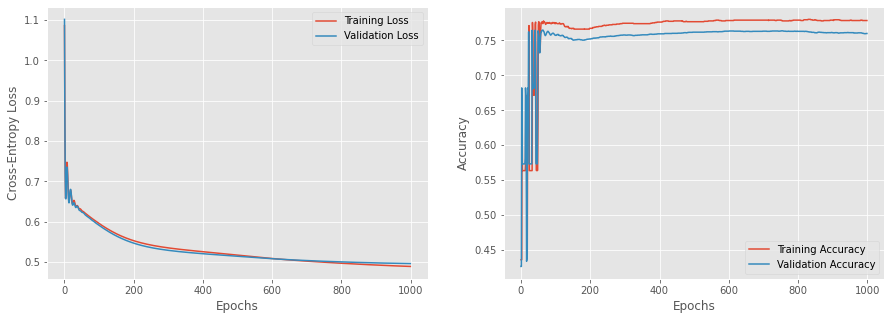
\includegraphics[width=0.9\textwidth]{gcn_plots.png}
		\caption{GCN Loss- and Accuracy Plots}
        \label{fig:gcn_plots}
  \end{figure}

  \noindent The confusion matrices and the final accuracies are shown in tables 
  \ref{table:gcn_results_train} \& \ref{table:gcn_results_valid}. 

  \begin{table}[h]
    \centering
    \begin{tabular}{|l|c|c|}
      \hline
      \diagbox{\textbf{Label}}{\textbf{Predicted}} & \textbf{Neutral or
      Dissatisfied} & \textbf{Satisfied}\\
      \hline
      \textbf{Neutral or Dissatisfied} & 776 & 232 \\\hline 
      \textbf{Satisfied} & 164 & 616 \\\hline\hline
      \textbf{Accuracy} & 77.85\% & \\
      \hline
    \end{tabular}
    \caption{Confusion Matrix Training Data GCN}
    \label{table:gcn_results_train}
  \end{table}

  \begin{table}[h]
    \centering
    \begin{tabular}{|l|c|c|}
      \hline
      \diagbox{\textbf{Label}}{\textbf{Predicted}} & \textbf{Neutral or
      Dissatisfied} & \textbf{Satisfied}\\
      \hline
      \textbf{Neutral or Dissatisfied} & 1'828 & 587 \\\hline 
      \textbf{Satisfied} & 424 & 1'372 \\\hline\hline
      \textbf{Accuracy} & 76.00\% & \\
      \hline
    \end{tabular}
    \caption{Confusion Matrix Validation Data GCN}
    \label{table:gcn_results_valid}
  \end{table}

  \noindent \acsp{gcn} are designed to be used in a transductive setting and the 
  model cannot be applied to new and unseen graphs. In this setting 30\% of the 
  dataset are used for training and 70\% of the data is used for validation. 
  This is done by masking the nodes in the graph which are part of the 
  validations dataset. The masked nodes are considered in the neighborhood 
  function $\mathcal{N}(v)$, they are just not considered as target nodes for 
  learning and updating the model parameters. The fact, that \acsp{gcn} cannot 
  be used in an inductive setting is very limiting. Further, the \acs{gcn} 
  requires 1'000 epochs to finish training and yields only mediocre results in 
  terms of accuracy and model fit. A reason for this could be, that only a 
  full batch implementation for \acs{gcn} was introduced. In addition,
  \acsp{gcn} always consider the entire neighborhood set. GraphSage for 
  comparison is specifically designed with mini-batch training and neighborhood 
  sampling in mind. The results for GraphSage are presented in the following 
  section. 

  \subsection{GraphSage}
  \label{section:graphsage_results}

  For GraphSage the exact same data input is used as for the \acs{gcn}. The 
  GraphSage model includes 2 convolutional layers with a hidden layer size of
  24 and an output layer size of 2. The model is defined using an adaptation of 
  algorithm \ref{algo:GraphSage}. Specifically, the hidden layer is activated 
  using the ReLU function with subsequent L2-normalization. The output of the 
  second layer is activated using the logsoftmax function. Normalization is 
  skipped for the final output. The training data is split into 80\% training 
  and 20\% validation using node masking. The loss is calculated using 
  cross-entropy and the model parameters are updated using the Adam optimizer 
  with the learning rate set to 0.002. The GraphSage model employed is thus an
  adaptation of the algorithm shown in algorithm \ref{algo:GNN_struct}. The 
  model is trained using a mini-batch size of 50 nodes and the neighborhood 
  function $\mathcal{N}(v)$ randomly samples 10 neighbors at a 2-hop distance
  from the target node and randomly samples 5 nodes at a 1-hop distance. This 
  corresponds to the steps shown in figure \ref{fig:GraphSage_sample}. To 
  improve the robustness of the model, a dropout rate of $p = 0.02$ is set. 
  GraphSage is run using the aggregation strategies mean, \acs{lstm},
  max-pooling, and sum-pooling. The model for each aggregation strategy is 
  trained using 400 epochs. The training- and validation results using the 
  training graph are presented for every aggregation strategy. In addition, 
  the trained models are applied to a new unseen test graph which also consists 
  of 6'000 randomly sampled nodes. The test graph is created analogues to the 
  training- and validation graph using a separate test feature dataset. The 
  results for all aggregation strategies are presented in the following 
  paragraphs. 

  \paragraph{Mean Aggregation}  \mbox{}\\ 
  In figure \ref{fig:mean_aggregation} the training- and validation losses as
  well as the accuracies for the mean aggregation model is shown.

  \begin{figure}[h]
		\centering
		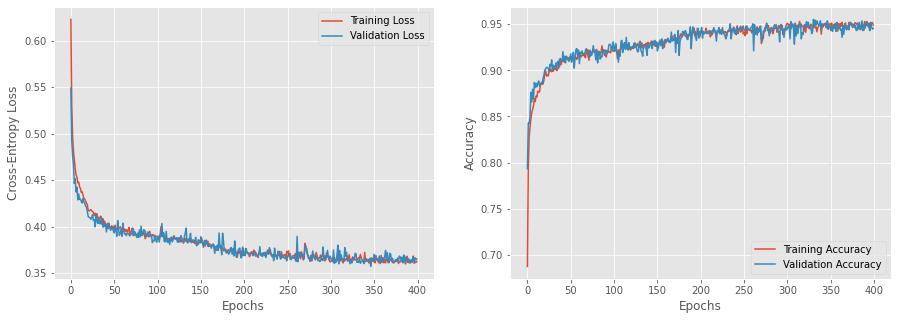
\includegraphics[width=0.9\textwidth]{graphsage_mean_plots.png}
		\caption{Mean Aggregation Loss- and Accuracy Plots}
        \label{fig:mean_aggregation}
  \end{figure}

  \noindent The training accuracy is 94.91\% and the validation accuracy is 
  94.80\% after training the model for 400 epochs. The loss- and accuracy plots
  show a good model fit which remains stable. The model resulted in a 
  test accuracy of 94.08\% with the confusion matrix shown in table
  \ref{table:mean_results_test}:

  \begin{table}[h]
    \centering
    \begin{tabular}{|l|c|c|}
      \hline
      \diagbox{\textbf{Label}}{\textbf{Predicted}} & \textbf{Neutral or
      Dissatisfied} & \textbf{Satisfied}\\
      \hline
      \textbf{Neutral or Dissatisfied} & 3'278  & 88 \\\hline 
      \textbf{Satisfied} & 267 & 2'367 \\\hline\hline
      \textbf{Accuracy} & 94.08\% & \\
      \hline
    \end{tabular}
    \caption{Test Confusion Matrix Mean Aggregation}
    \label{table:mean_results_test}
  \end{table}

  \paragraph{LSTM Aggregation}  \mbox{}\\ 
  Figure \ref{fig:lstm_aggregation} shows the training- and validation loss
  and the accuracy using LSTM aggregation. The model yields very good results 
  for the training- and validation data sets. The LSTM model is however 
  significantly slower for training purposes compared to the other aggregation 
  methods. This is an inconvenient short-coming.

  \begin{figure}[h]
		\centering
		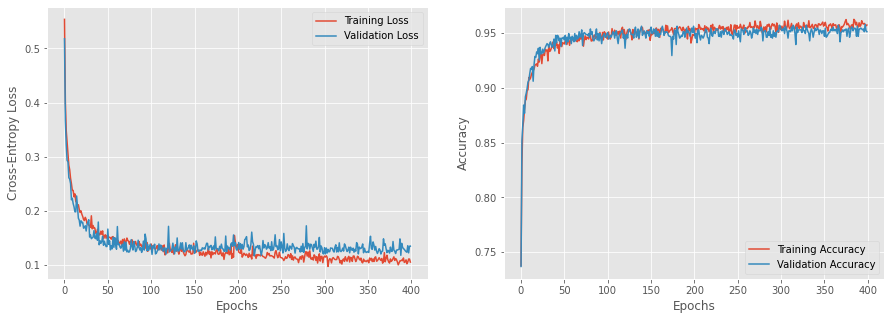
\includegraphics[width=0.9\textwidth]{graphsage_lstm_plots.png}
		\caption{LSTM Aggregation Loss- and Accuracy Plots}
        \label{fig:lstm_aggregation}
  \end{figure}

  \noindent The training- and validation accuracy after 400 epochs is 95.75\% 
  and 95.14\% respectively. Here again, it is shown that the training behavior
  is relatively good. The model is however prone to over-fit as shown in figure 
  \ref{fig:lstm_aggregation}. Fortunately, the over-fit is small and remains 
  stable. The results for the test graph are shown in table 
  \ref{table:lstm_results_test}. The results reveal, that the accuracies of >
  95\% for the training- and validation datasets do not transfer to the test
  graph. While this is to be expected, the decrease in accuracy for the test
  graph is most pronounced for \acs{lstm} aggregation. This further indicates, 
  that \acs{lstm} aggregation is prone to over-fitting.

  \begin{table}[h]
    \centering
    \begin{tabular}{|l|c|c|}
      \hline
      \diagbox{\textbf{Label}}{\textbf{Predicted}} & \textbf{Neutral or
      Dissatisfied} & \textbf{Satisfied}\\
      \hline
      \textbf{Neutral or Dissatisfied} & 3'288  & 78 \\\hline 
      \textbf{Satisfied} & 268 & 2'366 \\\hline\hline
      \textbf{Accuracy} & 94.23\% & \\
      \hline
    \end{tabular}
    \caption{Test Confusion Matrix LSTM Aggregation}
    \label{table:lstm_results_test}
  \end{table}

  \paragraph{Sum-Pooling Aggregation}  \mbox{}\\ 
  Sum-pooling is added for the reasons outlined in section
  \ref{section:theory_graphsage}. It is of particular interest to assess, 
  whether sum-pooling can provide some added value compared to the other 
  aggregation strategies. Given the feature data, sum aggregation is 
  unfortunately not injective. For that reason, it is not expected to 
  necessarily dominate the other strategies. Nevertheless, it is of interest to 
  assess, whether sum aggregation is competitive if not superior even in a 
  non-injective setting. The training- and validation results are shown in 
  figure \ref{fig:sum_aggregation}. 

  \begin{figure}[H]
		\centering
		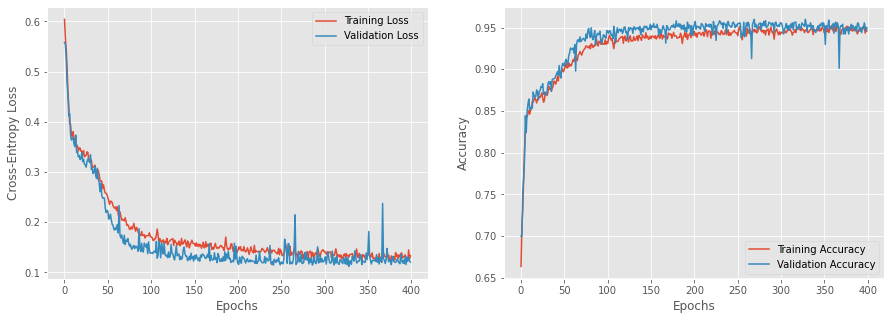
\includegraphics[width=0.9\textwidth]{graphsage_sum_plots.png}
		\caption{Sum-Pooling Aggregation Loss- and Accuracy Plots}
        \label{fig:sum_aggregation}
  \end{figure}

  \noindent The plots show that sum-pooling finishes with a good model fit. The
  loss curves are however not as smooth compared to the other aggregation
  strategies. After training for 400 epochs, the training accuracy is at 94.60\% 
  and validation accuracy is  94.97\%. The results for the test graph are shown 
  in table \ref{table:sum_results_test}. Sum-pooling yields competitive results,
  it does however not dominate the other aggregation strategies.

  \begin{table}[h]
    \centering
    \begin{tabular}{|l|c|c|}
      \hline
      \diagbox{\textbf{Label}}{\textbf{Predicted}} & \textbf{Neutral or
      Dissatisfied} & \textbf{Satisfied}\\
      \hline
      \textbf{Neutral or Dissatisfied} & 3'235  & 131 \\\hline 
      \textbf{Satisfied} & 213 & 2'421 \\\hline\hline
      \textbf{Accuracy} & 94.27\% & \\
      \hline
    \end{tabular}
    \caption{Test Confusion Matrix Sum-Pooling}
    \label{table:sum_results_test}
  \end{table}

  \paragraph{Max-Pooling Aggregation}  \mbox{}\\ 
  The training- and validation loss as well as the accuracies of max-pooling are 
  shown in figure \ref{fig:max_aggregation}. 

  \begin{figure}[h]
		\centering
		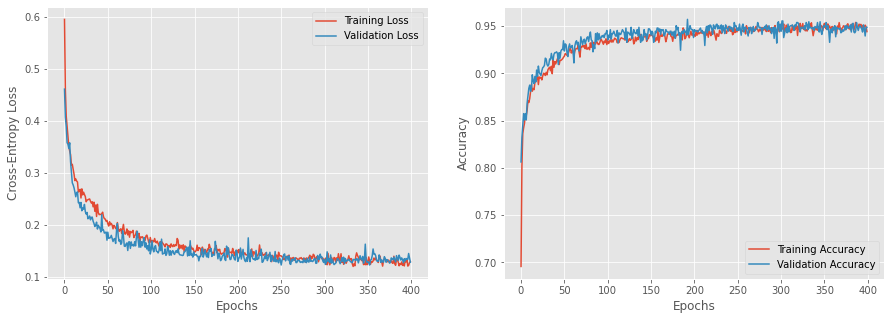
\includegraphics[width=0.9\textwidth]{graphsage_max_plots.png}
		\caption{Max-Pooling Aggregation Loss- and Accuracy Plots}
        \label{fig:max_aggregation}
  \end{figure}

  \noindent After 400 epochs, the model arrived at a training accuracy of 94.43\% 
  and a validation accuracy of 94.88\%. The results for the test graph are shown 
  in table \ref{table:max_results_test}. Max-pooling yields the best results and
  corresponds to the recommended method by \citeauthor{hamilton2017inductive} 
  \citeyearpar[p. 9]{hamilton2017inductive}.

  \begin{table}[h]
    \centering
    \begin{tabular}{|l|c|c|}
      \hline
      \diagbox{\textbf{Label}}{\textbf{Predicted}} & \textbf{Neutral or
      Dissatisfied} & \textbf{Satisfied}\\
      \hline
      \textbf{Neutral or Dissatisfied} & 3'235  & 131 \\\hline 
      \textbf{Satisfied} & 212 & 2'422 \\\hline\hline
      \textbf{Accuracy} & 94.28\% & \\
      \hline
    \end{tabular}
    \caption{Test Confusion Matrix Max-Pooling}
    \label{table:max_results_test}
  \end{table}

  \subsection{GraphSage Robustness Simulation}
  \label{section:graphsage_simulation}
  
  The loss- and accuracy plots using the GraphSage model reveal mostly a 
  relatively good model fit. Repeatedly training the GraphSage models revealed, 
  that there is some non-negligible variation in the performance of the trained 
  models. In particular, depending on how the data is randomly split into 80\% training
  data and 20\% validation data, the model results could differ significantly.
  Simulations reveal, that the random assignment of training- and validation
  data is not the sole culprit for the observed variation in model performance. 
  The dropout rate of 2\% employed in the GraphSage model is just as responsible. 
  Simulations show, that if the dropout rate is set to 0, that the model tends
  to over-fit significantly. In this setting, the training accuracy approaches
  98\% while the validation accuracy stagnates around 92-93\%. The trained model 
  accordingly does not translate well to the test graph for which the accuracy
  is approximately 91\%. This training behavior is observed regardless of the
  random train- and validation data set assignment. For that reason, a dropout 
  rate of 2\% is set to avoid this over-fitting problem which in turn also 
  yields better test results as shown in section \ref{section:graphsage_results}. \\

  \noindent Setting a dropout rate introduces an additional obstacle
  for training the model. While training the model, the dropout rate is
  applied for forward propagating the training data. The validation data is 
  however forward propagated with no dropout. This is the intended mechanism
  which can be used to prevent over-fitting. This however makes the model more
  sensitive to the random assignment of nodes into training- and validation
  data. Given the structure present in the graph, some nodes are more difficult
  to classify than others. If the training data includes more difficult nodes
  in combination with the dropout rate, the outcome can occur where the
  validation data has a lower loss and a higher accuracy than the training
  data. The same can be true in reverse, where an over-fit occurs if the
  training data includes mostly nodes which are more simple to classify than
  the validation data. Lastly, a good model fit is also frequently observed as
  shown in the results presented in the previous section. \\

  \noindent Due to this observed variation in model fit and performance, a
  simulation is performed with 100 experiments. Every experiment makes use of
  the same training \& validation graph and test graph. For every experiment,
  the training- and validation set is randomly assigned using a 80/20 split.
  Afterwards, the model is trained using 400 epochs and is then applied to the
  test graph. The loss and accuracy for the training, validation and test data
  is collected for every experiment. These experiments are conducted to
  ensure, that the results shown in section \ref{section:graphsage_results} are
  representative. The results of the 100 experiments using GraphSage with
  max-pooling is shown in table \ref{table:simulation_results} and figure 
  \ref{fig:simulation_results}. 

  \begin{table}[h]
    \centering
      \begin{tabular}{|l||c|c|c|}
      \hline
      \textbf{Metric} & \textbf{Training Set} & \textbf{Validation Set} & 
      \textbf{Test Set}\\
      \hline\hline
      Average Accuracy & 94.95\% & 94.90\% & 93.79\% \\\hline 
                       & (0.65\%) & (0.75\%) & (0.41\%) \\\hline
      Average Cross-Entropy Loss & 0.1276 & 0.1313 & 0.1625 \\\hline
                                 & (0.0140) & (0.0170) & (0.0108) \\
      \hline
    \end{tabular}
    \caption{Simulation Results Max-Pooling}
    \label{table:simulation_results}
  \end{table}

  \begin{figure}[htbp!]
		\centering
		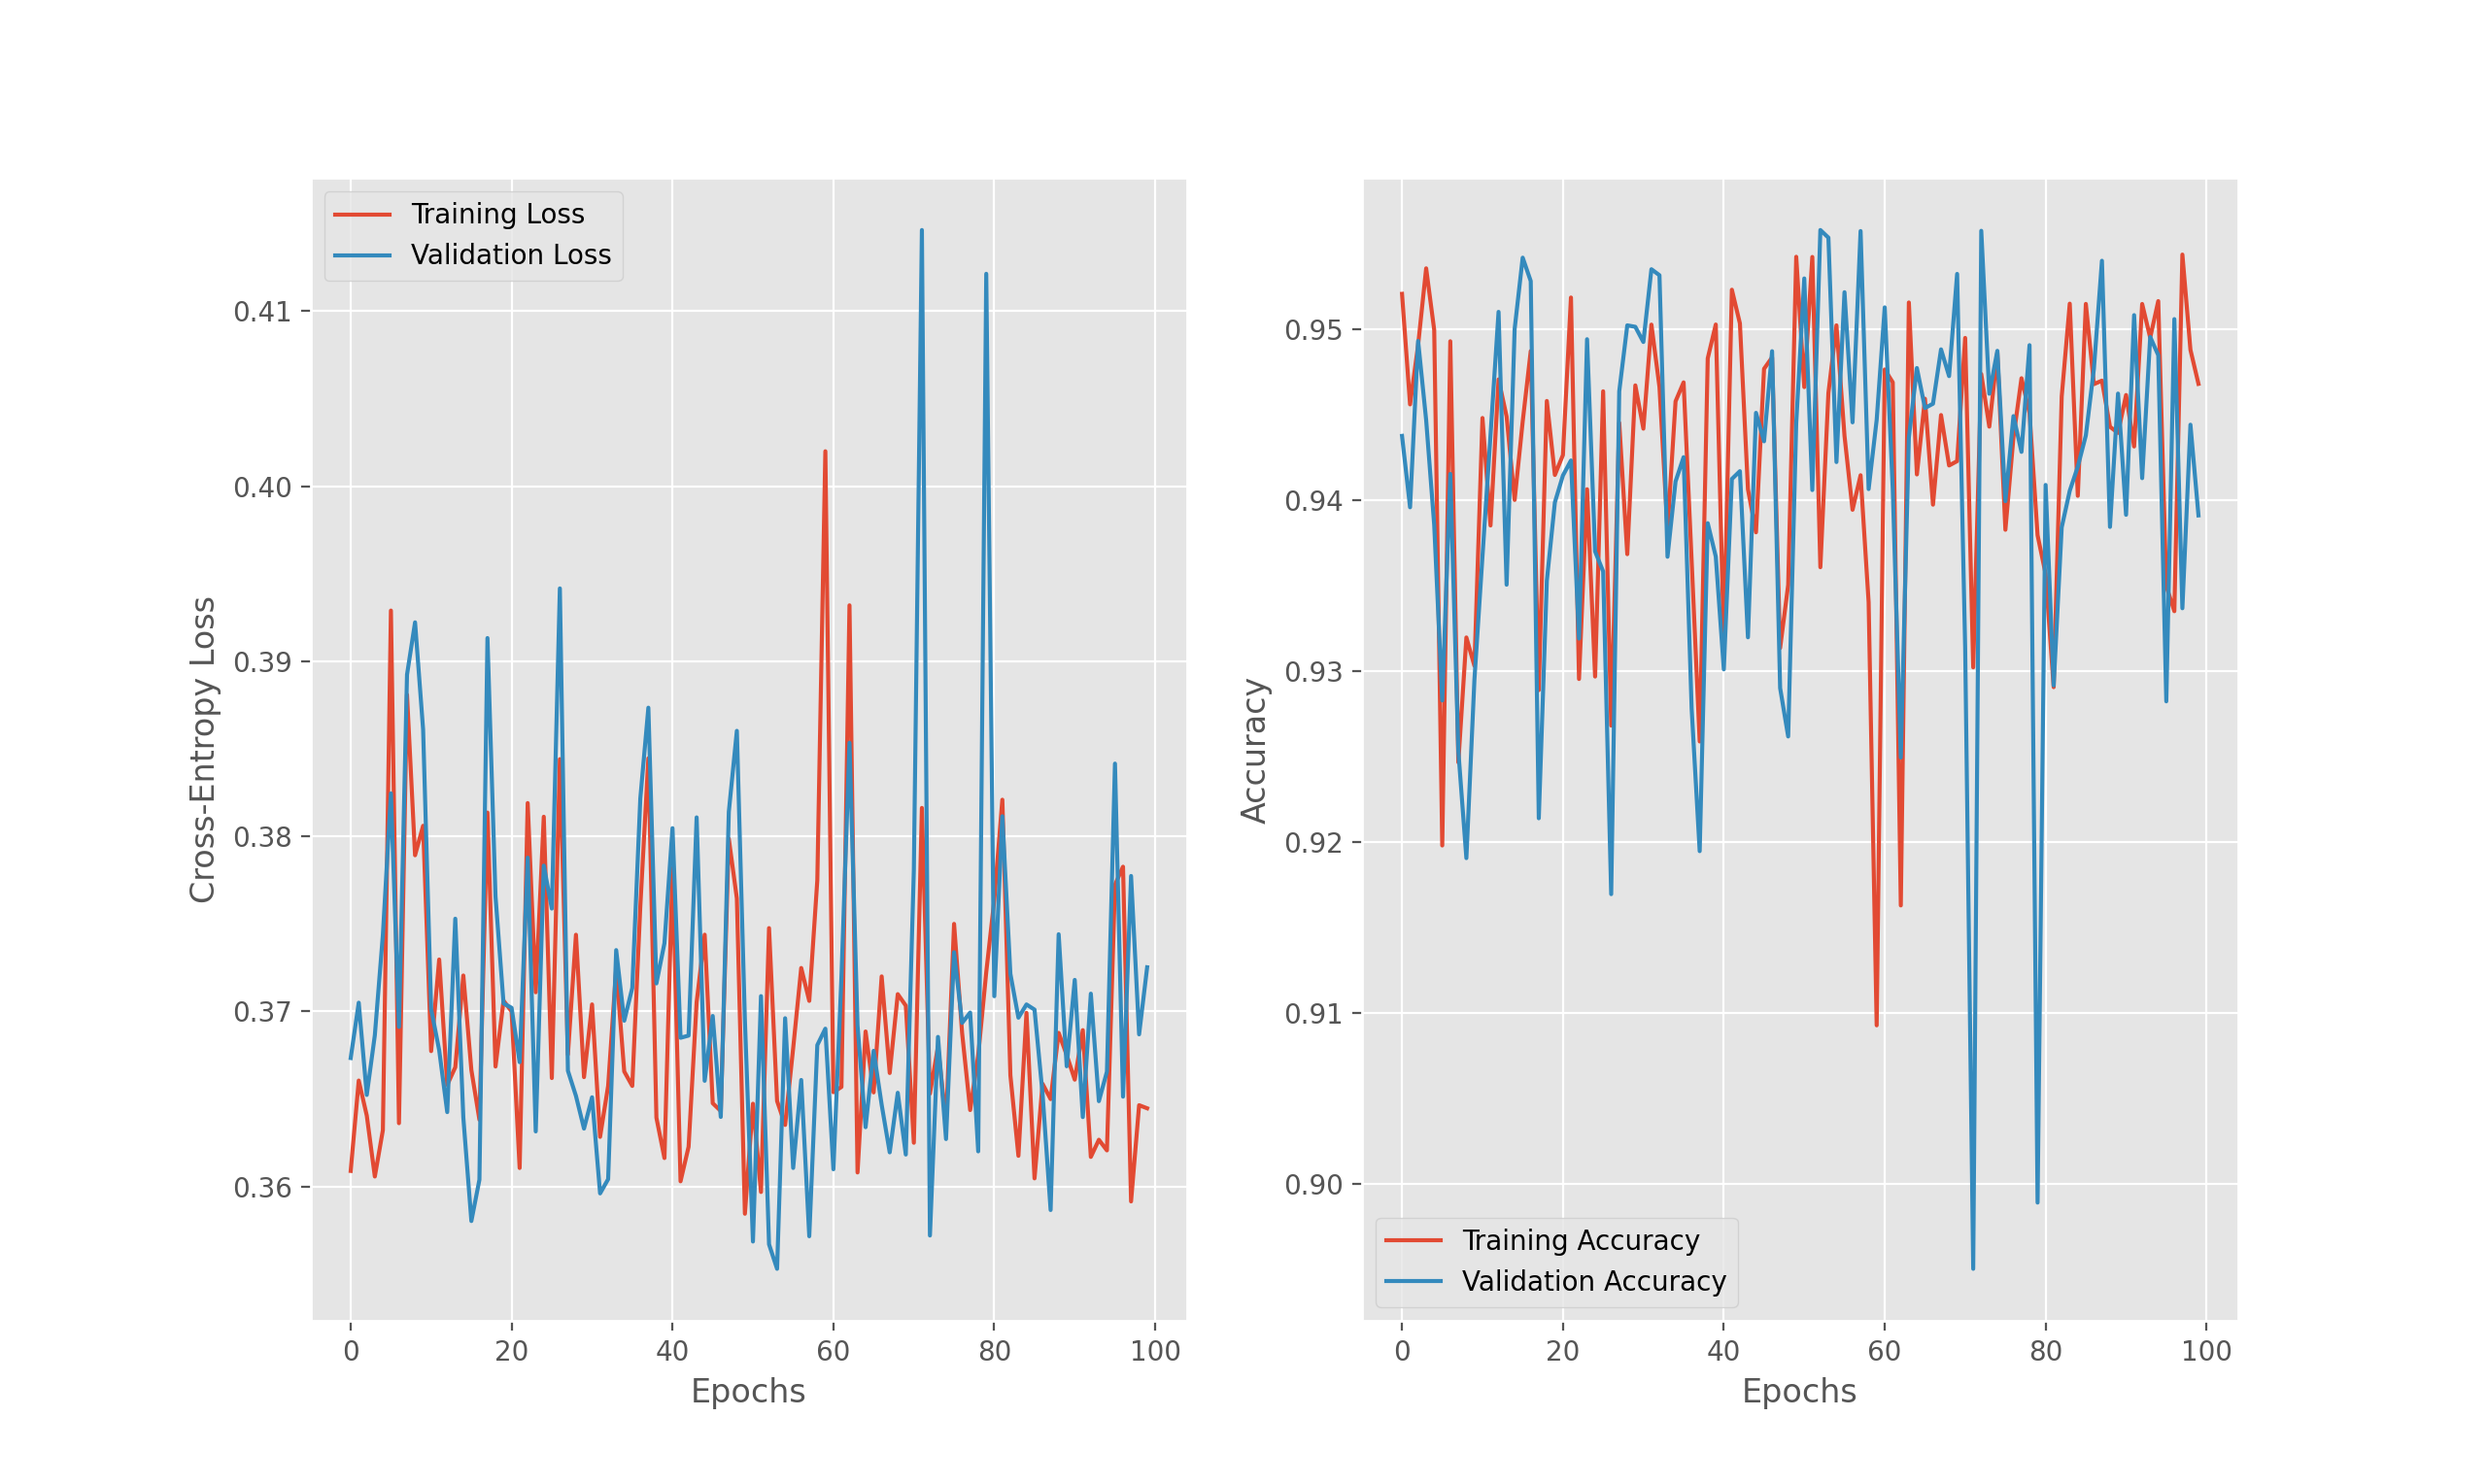
\includegraphics[width=1.0\textwidth]{max_100_sim.png}
		\caption{Simulation Results Max-Pooling}
        \label{fig:simulation_results}
  \end{figure}

  \noindent Max-pooling is selected as it corresponds to the recommended
  aggregation strategy \citep[p. 9]{hamilton2017inductive}. The same simulation
  using 100 experiments is also performed for sum-pooling. The results are
  almost identical, where max-pooling is marginally more successful. For the 
  remaining aggregation strategies, only 10 experiments are run due to time
  considerations as 100 experiments require approximately 15 hours to complete.
  The required time for the simulation could most definitely be shortened using
  a \ac{gpu}. Unfortunately, a \acs{gpu} is not available for conducting the 
  simulations. If available, this would be highly recommended to shorten the 
  required time for completing the simulations. The results using only 10 
  experiments yields similar results, with test accuracies ranging mostly 
  between 93-94\%. The simulation results for mean, \acs{lstm} and sum aggregation 
  are shown in appendix \ref{App:sim_results}. The results shown in section 
  \ref{section:graphsage_results} are therefore representative results, even if 
  admittedly on the more positive side. 

  \section{Result Comparison}
  \label{section:result_comp}

  This section compares the results of the three models Node2Vec, \acs{gcn} and
  GraphSage. In addition the graph based \acs{ml} models are compared to the 
  standard \acs{ml} models. More precisely, the same standard \acs{ml} models 
  are used for comparison as for the downstream \acs{ml} task for \acs{grl} 
  shown in section \ref{section:result_n2v}. For the comparison, the standard 
  \acs{ml} models consider the same features as inputs as the \acsp{gnn}. The 
  comparison is done to assess to what extent, semi-synthetic graphs are useful 
  for \acs{gml}. This comparison thus provides the key results for answering
  the research question and assessing the hypotheses stated in section 
  \ref{section:research_topics}. The comparison of the results is shown in table 
  \ref{table:result_comparison}.

  \begin{table}[h]
    \centering
    \scalebox{0.79}{
      \begin{tabular}{|l||c|c|c|}
      \hline
      \textbf{Method} & \textbf{Training Accuracy} & \textbf{Validation
      Accuracy} & \textbf{Test Accuracy}\\
      \hline\hline
      Logistic Regression & 87.94\% & 87.17\% & 86.77\% \\\hline 
      Naive Bayes & 87.50\% & 86.17\% & 85.82\% \\\hline
      QDA & 70.5\% & 70.00\% & 69.23\% \\\hline
      AdaBoost & 94.06\% & 92.33\% & 93.00\% \\\hline
      Random Forest & 100\% & 94.42\% & 94.55\% \\\hline
      SVM & 94.65\% & 92.25\% & 92.73\% \\\hline
      ANN & 94.86\% & 95.00\% & 93.13\%\\\hline
      Node2Vec (Logistic Regression) & 77.04\% & 76.16\% & 57.06\% \\\hline
      GCN & 77.85\% & 76.00\% & -\\\hline
      GraphSage (Mean Aggregation) & 94.91\% & 94.80\% & 94.08\% \\\hline
      GraphSage (LSTM Aggregation) & 95.75\% & 95.14\% & 94.23\% \\\hline
      GraphSage (Sum-Pooling) & 94.60\% & 94.97\% & 94.27\% \\\hline
      GraphSage (Max-Pooling) & 94.43\% & 94.88\% & 94.28\% \\
      \hline
      \end{tabular}}
    \caption{Result Comparison}
    \label{table:result_comparison}
  \end{table}

  \noindent The results for the \acs{gml} models shown in table 
  \ref{table:result_comparison} correspond to the results shown in sections
  \ref{section:result_n2v}, \ref{section:GCN_results} and 
  \ref{section:graphsage_results}. For \acs{grl} (Node2Vec), the results using 
  logistic regression for downstream \acs{ml} are shown. This method is selected, 
  as it provides the best overall results in terms of accuracy and model simplicity. \\

  \noindent The comparison shown in table \ref{table:result_comparison} reveals,
  that \acsp{gcn} and Node2Vec are not competitive strategies for the \acs{us} 
  airline passenger dataset. GraphSage is shown to be a serious competitor and 
  is the second best model. The Random Forest classifier is consistently the best 
  model regardless of the training- and validation data split and test data. 
  The \acs{ann} is the third best model and is only marginally inferior to the
  GraphSage models. Similarly as for \acsp{gnn}, it is important to evaluate the 
  model fit of the \acs{ann} to draw a more definitive conclusion. The loss- and
  accuracy plots of the \acs{ann} are shown in figure \ref{fig:ANN_fit}.

  \begin{figure}[h]
		\centering
		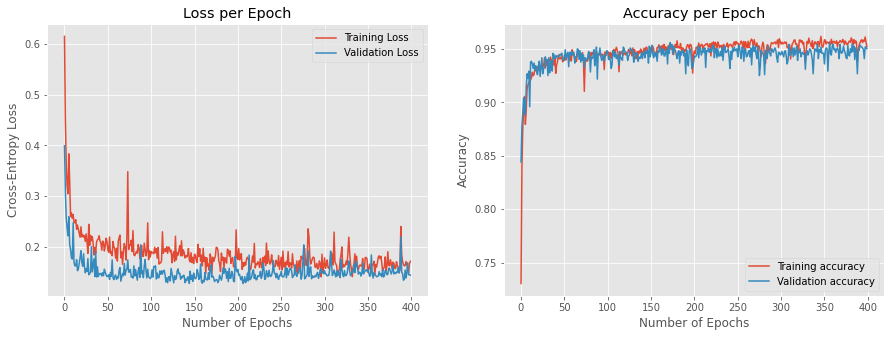
\includegraphics[width=0.9\textwidth]{ANN_Plot.png}
		\caption{ANN Model Fit}
        \label{fig:ANN_fit}
  \end{figure}

  \noindent The \acs{ann} has an input layer size of 24, a hidden layer size of 
  15 and an output layer with size 2. The output of the first layer is activated
  using the ReLU function and the output of the second layer is activated
  using the softmax function. The loss is calculated using cross-entropy and
  the model parameters are updated using the Adam optimizer with a learning
  rate of $\alpha=0.002$. The dropout rate is set to $p=0.01$. Without setting 
  the dropout rate, the \acs{ann} is prone to significant over-fitting. The 
  presented model settings correspond to the ones which performed best for the 
  \acs{ann}. Figure \ref{fig:ANN_fit} shows, that the \acs{ann} model starts 
  over-fitting after approximately 200 epochs. When comparing the GraphSage 
  training plots with the \acs{ann}, the GraphSage model appears to exhibit 
  preferable training behavior on average. \\

  \noindent AdaBoost and \acs{svm} also are shown to yield good results. The test
  accuracies are however not as competitive compared to the previously
  mentioned methods. Lastly naive bayes, \acs{qda} and logistic regression clearly
  yield inferior results. 
